\chapter{Metodolog�a}

\section{Generalidades}

Debido a la naturaleza del tema, el curso tendr� un componente te�rico en el que se dar�n las bases conceptuales del t�pico a tratar, para posteriormente realizar laboratorios pr�cticos con el fin de afianzar los conocimientos. La mayor parte de las pr�cticas se realizar�n con la tarjeta de desarrollo AndroidStamp presentada con anterioridad (ver figura \ref{stamp}). Algunas otras pr�cticas se desarrollar�n con plataformas especiales para validar ejemplos presentados en clase, tal como el uso de dispositivos FPGA o microcontroladores.

%\begin{figure}[htp]
%    \begin{center} 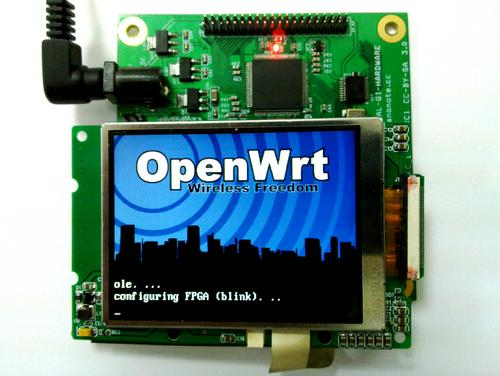
\includegraphics[scale=0.4]{images/SAKC_DC.jpg}\end{center}
%    \begin{center} 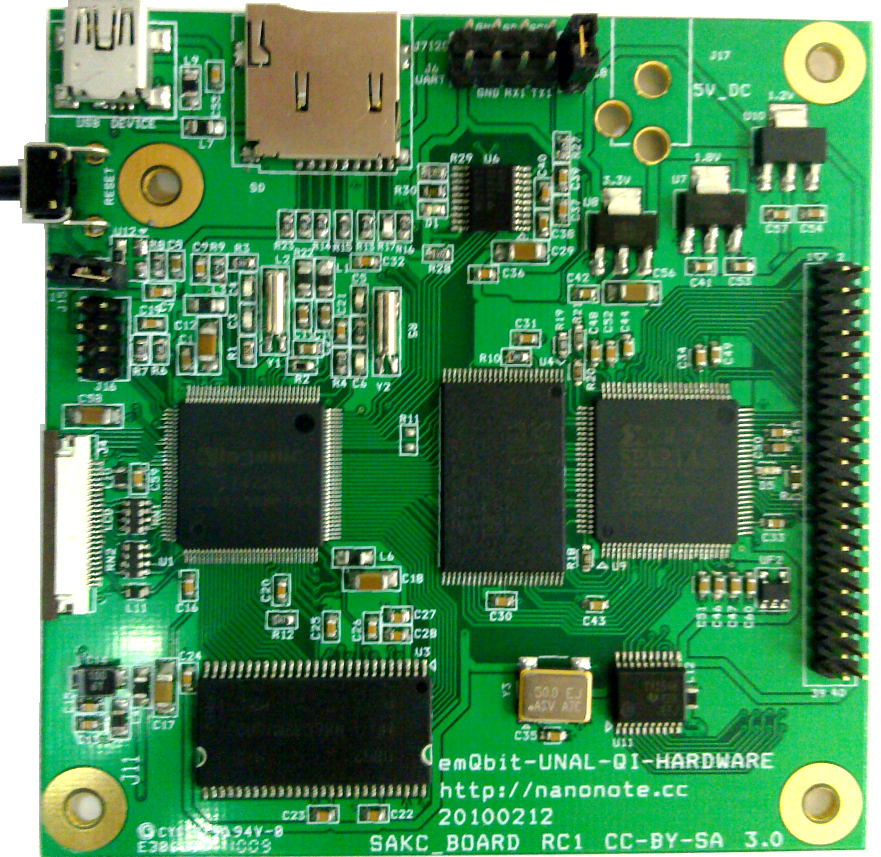
\includegraphics[scale=0.4]{images/Sakc.png}\end{center}
% \caption{Plataforma de Desarrollo stamp}
%  \label{stamp}
%\end{figure}

Es de vital importancia la participaci�n activa de los asistentes en todas las actividades del diplomado para as� garantizar la utilidad del mismo. Los inscritos que realicen el 90\% de las actividades propuestas recibir�n una certificaci�n por parte de la Universidad Nacional de Colombia.


\section{Duraci�n}
El curso tendr� una intensidad horaria de 100 horas.


\section{Dirigido A}
El diplomado en ``Herramientas Modernas para Dise�o y Fabricaci�n de Dispositivos Digitales'' est� dirigido a estudiantes y profesionales en todas las �reas relacionadas con la ingenier�a el�ctrica, electr�nica, de computadores, sistemas, telecomunicaciones, rob�tica y mecatr�nica, o similares.

Los participantes del diplomado podr�n reforzar sus conocimientos en t�cnicas de dise�o de sistemas digitales, y al mismo tiempo, podr�n actualizarse en el uso de nuevos tecnolog�as en esta importante �rea de la electr�nica.


